% Copyright 2007-2024 Joakim Nilsson
%
% This file is part of Combo Whist.
%
% Combo Whist is free software: you can redistribute it and/or modify
% it under the terms of the GNU General Public License as published by
% the Free Software Foundation, either version 3 of the License, or
% (at your option) any later version.
%
% Combo Whist is distributed in the hope that it will be useful,
% but WITHOUT ANY WARRANTY; without even the implied warranty of
% MERCHANTABILITY or FITNESS FOR A PARTICULAR PURPOSE.  See the
% GNU General Public License for more details.
%
% You should have received a copy of the GNU General Public License
% along with Combo Whist.  If not, see <http://www.gnu.org/licenses/>.

\documentclass[a4paper]{article} % Document class
\usepackage[english]{babel}                         % Language
\newcommand{\dash}{---}                             % Language-dependent dash
\newcommand{\specialBidText}{Special~Bid}           % Special bid text
\newcommand{\standardBidText}{Standard~Bid}         % Standard bid
\newcommand{\nonTrump}{\textnormal{non-trump bids}} % Non-trump bids text
          % Language-dependent code
% Copyright 2007-2022 Joakim Nilsson
%
% This file is part of Combo Whist.
%
% Combo Whist is free software: you can redistribute it and/or modify
% it under the terms of the GNU General Public License as published by
% the Free Software Foundation, either version 3 of the License, or
% (at your option) any later version.
%
% Combo Whist is distributed in the hope that it will be useful,
% but WITHOUT ANY WARRANTY; without even the implied warranty of
% MERCHANTABILITY or FITNESS FOR A PARTICULAR PURPOSE.  See the
% GNU General Public License for more details.
%
% You should have received a copy of the GNU General Public License
% along with Combo Whist.  If not, see <http://www.gnu.org/licenses/>.

% Document class
\documentclass[a4paper]{article}

\usepackage[swedish]{babel}
% Copyright 2014-2020 Joakim Nilsson
%
% This file is part of Combo Whist.
%
% Combo Whist is free software: you can redistribute it and/or modify
% it under the terms of the GNU General Public License as published by
% the Free Software Foundation, either version 3 of the License, or
% (at your option) any later version.
%
% Combo Whist is distributed in the hope that it will be useful,
% but WITHOUT ANY WARRANTY; without even the implied warranty of
% MERCHANTABILITY or FITNESS FOR A PARTICULAR PURPOSE.  See the
% GNU General Public License for more details.
%
% You should have received a copy of the GNU General Public License
% along with Combo Whist.  If not, see <http://www.gnu.org/licenses/>.

%==========
% Packages
%==========

\usepackage[utf8]{inputenc}
\usepackage[protrusion=true]{microtype} % More readable layout
\usepackage{graphicx}                   % \rotatebox
\usepackage{tabularx}                   % X column specifier in tables
\usepackage[pass]{geometry}             % Changing margins
\usepackage[labelfont=bf]{caption}      % Captions boldface
\usepackage{siunitx}                    % Number alignment in tables
\usepackage{xfrac}                      % Vulgar fractions
\usepackage{verbatim}                   % Monospaced text
\usepackage[
	ocgcolorlinks=true,
	urlcolor={[rgb]{0,0,1}},
	linkcolor={[rgb]{0.4,0,0}},
]{hyperref}

%======================================
% Include makefile generated variables
%======================================

\input{tmp/vars.tex}

%==========
% Commands
%==========

% Rotate text 90 degrees
\newcommand{\rotccw}[1]{%
	\rotatebox{75}{{#1}}
}

\newcommand{\standardBidItem}[6]{%
	\\ \hline
	\textit{#1} &
	#2 &
	#3 &
	#4 &
	#5 &
	\small #6
}

\newcommand{\specialBidItem}[4]{%
	\\ \hline
	\textit{#1} &
	#2 &
	\raggedright\textit{#3} &
	\small #4
}

\newcommand{\nonTrump}{\textnormal{non-trump bids}}

\newcommand{\introPages}{%
	\maketitle

	\vfill

	% Logo
	\begin{center}
		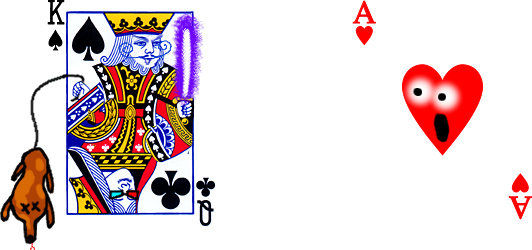
\includegraphics[width = \textwidth]{../logo.png}
	\end{center}

	\vfill

	% License
	% This file is part of Combo Whist.
%
% Copyright 2014-2019 Joakim Nilsson
%
% This file is part of Combo Whist.
%
% Combo Whist is free software: you can redistribute it and/or modify
% it under the terms of the GNU General Public License as published by
% the Free Software Foundation, either version 3 of the License, or
% (at your option) any later version.
%
% Combo Whist is distributed in the hope that it will be useful,
% but WITHOUT ANY WARRANTY; without even the implied warranty of
% MERCHANTABILITY or FITNESS FOR A PARTICULAR PURPOSE.  See the
% GNU General Public License for more details.
%
% You should have received a copy of the GNU General Public License
% along with this text.  If not, see <http://www.gnu.org/licenses/>.
% License notice

\begin{verbatim}
	Copyright 2007-2019 Joakim Nilsson

	This document is part of Combo Whist.

	Combo Whist is free software: you can redistribute it and/or modify
	it under the terms of the GNU General Public License as published by
	the Free Software Foundation, either version 3 of the License, or
	(at your option) any later version.

	Combo Whist is distributed in the hope that it will be useful,
	but WITHOUT ANY WARRANTY; without even the implied warranty of
	MERCHANTABILITY or FITNESS FOR A PARTICULAR PURPOSE.  See the
	GNU General Public License for more details.
\end{verbatim}
\verb|You should have received a copy of the GNU General Public License|\\
\verb|along with this text.  If not, see <|\url{http://www.gnu.org/licenses/}\verb|>.|


	\thispagestyle{empty}
	\pagebreak

	% Table of contents and list of tables without protrusion
	\microtypesetup{protrusion=false}
	\setcounter{tocdepth}{3}
	\tableofcontents
	\listoftables
	\microtypesetup{protrusion=true}
	\thispagestyle{empty}
	\pagebreak
}


% Title
\defTitle{Kombinations-Whist}{Det Obesudlade Kortspelet}

% Links text
\defLinks{För den senaste versionen av reglerna, besök \rulesUrl\ eller prenumerera på \rssUrl.}

% Author
\author{Av Joakim Nilsson}

% Date and version
\ifdefined\varDev
	\date{Utvecklingsversion (baserad på version \varVersion-\varLanguage)---\today}
\else
	\date{Version \varVersion-\varLanguage\---\today}
\fi

% Document
\begin{document}
	%=============
	% Intro pages
	%=============

	\introPages
	\pagebreak

	%======
	% Body
	%======

	\section{Översikt}
		Kombinations-Whist är ett kortspel som bygger på sticktagande och är---som namnet antyder---en variant av Whist. Kombinations-Whists nyckelegenskap är dess varierade utbud av möjliga strategier med acceptabelt simpla regler. (Det måste dock erkännas att regelboken trots allt är någorlunda lång.) Möjligheten att spela enligt många varierade strategier undviker en substantiell mängd slump som vanligtvis finnes i andra Whist-spel utan att att göra spelet alltför komplicerat. Detta gör Kombinations-Whist till ett spel som är kul att spela både för erfarna spelare såväl som för nybörjare.

		\paragraph{Antal spelare:}
		4 är att föredra, men 3 till $\infty$ går också bra med vissa regeljusteringar.

		\paragraph{Vad som behövs för att spela:}
		En standard-kortlek med 52 kort samt penna och papper.

		\paragraph{Kortens rang:}
		Från högst till lägst: E, K, D, Kn, 10, 9, 8, 7, 6, 5, 4, 3, 2

	\section{Hur man spelar}
		\subsection{Förberedelser}
			Gör en kolumn för varje spelare på pappret. Detta för att hålla koll på poängställningen samt lite annan information om spelet. När pappret har förberetts, slumpa då fram vem som blir giv.

			Om det bara finns 3 spelare, ta ut $\clubsuit 6$, samt alla 7:or, 8:or och 9:or från leken.

		\subsection{Given}
			Det finns två huvudsakliga delar av en giv. Den första är \emph{budgivningen} och den andra är \emph{spelet}. Eftersom det borde bli lättare att förstå dessa två delar i omvänd ordning beskrivs spelet före budgivningen.

			En giv börjar med att given delar ut 13 kort till varje spelare. Därefter börjar budgivningen och när den är avklarad börjar spelet.

			Efter spelet noteras spelarnas poäng och en ny giv börjar där spelaren till vänster om den föregående given blir ny giv.

			\subsubsection{Spelet}
				Spelet spelas likt de flesta Whist-varianter. Spelaren till höger om \emph{spelföraren}\footnote{Begreppet ''spelförare'' förklaras i Stycke~\sectionref{bidding}.} börjar med att spela ut ett kort. Sen blir det spelaren till höger om denne som spelar ut nästa kort som dessutom måste följa färg. Därefter spelar näste spelare (till vänster om föregående) ut ännu ett kort som också måste följa det första kortets färg och så vidare till det att alla spelare har spelat ut ett kort vardera.

				Om en spelare har slut kort i den först utspelade färgen får denne saka valfritt kort eller spela en trumf. Till skillnad från många Whist-varianter finns inget trumftvång.

				Den spelare som spelade det högsta kortet i den först utspelade färgen tar hem \emph{sticket} (det vill säga, tar alla utspelade kort och lägger på bordet dem med bildsidan nedåt) såvida ingen har spelat ut en trumf. Om så skulle vara fallet är det den spelare som har spelat ut den högsta trumfen som tar hem sticket. Den spelare som tog hem det senaste sticket spelar ut först i nästa.

			\subsubsection{Budgivningen}
				\label{sec:bidding}
				I Kombimations-Whist budar man med \emph{kombinations-bud}. Ett kombinationsbud består av precis ett standardbud och en valfri mängd (inklusive noll) specialbud. Buden har särskilda regler förknippade med dem, vilka appliceras under spelet och poängberäkningen.

				Spelarna budar medsols och spelaren till vänster om given börjar. En spelare kan antingen passa eller buda ett kombinationsbud som är värt mer än föregående kombinationsbud (som vi från och med nu helt enkelt kommer att kalla \emph{bud}). Om en spelare passar är denne ute ur budgivningen och får därför inte göra några nya bud förrän nästa giv. Om alla spelare passar blir det omgiv där samme giv ger igen.

				Ett buds värde definieras som det kombinerade värdet av standard- och specialbudet som det består av. För att ett bud ska få budas måste det ha ett värde av minst 1. Det föreslås att en tidsgräns på 20 sekunder sätts mellan varje bud och 1 minut före det första budet. För nybörjare är dock längre eller inga tidsgränser rekommenderade. Om en spelare inte har lagt ett bud inom den givna tiden så passar denne automatiskt. Budgivningen fortsätter fram till att alla spelare förutom en har passat. Den spelaren utnämns till spelförare och spelet börjar.

				De standardbud och specialbud som finns att tillgå finns listade i tabellerna i Stycke~\sectionref{standardBids} samt Stycke~\sectionref{specialBids}. Antalet stick att ta hem för att ett bud ska gå hem listas i standardbudstabellens ''Stick''-kolumn. Ett specialbud kan inte kombineras med ett annat bud som finns listade i ''Inkompatibilitet''-kolumnen. För övrigt är kombinationsbud som omöjligen kan gå hem oavsett motspelarnas kortfördelning förbjudna. Notera att det finns en skillnad mellan värde och poäng; Värde är budets värde (Rätt gissat!) och poäng är antalet poäng som spelföraren får om dennes bud går hem.

				Om det är oklart när en händelse som inträffar på grund av ett bud ska ske, se specialbudens ''Ordning''-kolumn. Ett buds ordning bestämmer i vilken ordning de olika händelserna som ges av dess regler ska ske. De bud med lägst ordning går först. Alla standardbud har ordningen 0.

			\subsubsection{Poängberäkningen}
				Efter att spelet är klart får spelföraren ett antal poäng baserat på vilket kombinationsbud som lagts och huruvida detta bud gick hem. Om budet gick hem får spelföraren det antal poäng som specificeras ''Poäng''-kolumnen för standardbudet. Om budet inte gick hem så förlorar spelföraren 2 poäng. En spelare kan anta en negativ poängsumma. Om en spelare antar en poängsumma lägre än $-5$, så tillåts denne inte längre att buda i budgivningar. Denne får dock 1 gratispoäng efter varje giv som denne deltar i (även om ingen budar och det blir omgiv).

			\subsubsection{Vem som vinner}
				\label{sec:winning}
				Det finns två varianter av hur man bestämmer vem som vinner i Kombinations-Whist: \emph{klassisk} och \emph{begränsad}.

				\paragraph{Klassisk:}
					Den som först uppnår eller överstiger \emph{vinstsumman} vinner. Vinstsumman börjar på 13, men minskar med 1 varje gång alla spelare har varit giv en gång vardera fram tills dess att vinstsumman går ned till 1. Vinstsumman minskar \emph{efter} att den sista given har spelats och poängen för den given har räknats. En spelare kan endast vinna genom att ett bud går hem och kan därför inte vinna enbart därför att vinstsumman just minskade. En spelare kan inte heller vinna om denne inte har enskilt flest poäng.

				\paragraph{Begränsad:}
					Ett förutbestämt antal \emph{rundor} spelas (förslagsvis 3), där en runda innefattar att alla spelare har varit giv en gång vardera. När rundorna har spelats vinner näste spelare som går hem med ett bud som resulterar i att denne uppnår enskilt flest poäng. För att förtydliga: En spelare kan vinna i samband med att sista rundan just spelats färdigt.

				\paragraph{Skamvinst} Gemensamt för bägge varianterna gäller att om alla spelare utom en innehar $-5$ poäng eller färre så vinner den spelare som har flest poäng automatiskt. Detta sätt att vinna kallas en \emph{Skamvinst}.

	\section{Övrigt}
		\subsection{Regler för fler än 4 spelare}
			Om fler är 4 spelare deltar i spelet så får alla utom 4 sitta ut (avstå att delta) i varje giv. De spelare som sitter ut är de som sitter närmast till höger om given.
		
		\subsection{Prat}
			En viss mängd av prat tillåts i Kombinations-Whist, men spelarna får inte ge ledtrådar om vad de har för kort.
		
		\subsection{Fusk}
			Om spelföraren oavsiktligen fuskar går nuvarande bud inte hem. Om en icke-spelförare fuskar händer följande: Det nuvarande budet spelas klart, men inget poängavdrag görs från spelförarens poängsumma utifall budet inte går hem. Dessutom dras samma antal poäng som det nuvarande budets poäng av från den fuskande spelarens poängsumma oavsett om budet går hem.

			Om oavsiktligt fusk inträffar innan en spelförare har utnämnts avbryts given och 2 poäng dras av från den fuskande spelarens poängsumma.

			Om givens samtliga spelare emellertid är överens om hur händelserna efter fusket inträffade ska återställas ska dock detta ske utan andra förändringar i poängsummorna förutom att 1 poäng dras av från den fuskande spelarens poängsumma.

			En spelare som avsiktligen fuskar i Kombinations-Whist får aldrig mer spela det eftersom denne uppenbarligen inte respekterar spelets prakt.

	%============
	% Bid tables
	%============

	\pagebreak
	\newgeometry{left=1cm, right=1cm, top=1cm}

	\section{Standardbud}
		\label{sec:standardBids}
		\begin{center}
			\begin{tabularx}{\textwidth}{
				p{2.5cm}
				S[table-number-alignment=center, table-format=1.0]
				S[table-number-alignment=center, table-format=1.0]
				ccX
			}
					\textbf{B\scriptsize ENÄMNING} &
					\rotccw{\textbf{Värde}} &
					\rotccw{\textbf{Poäng}} &
					\rotccw{\textbf{Trumf}} &
					\rotccw{\textbf{Stick}} &
					\textbf{Regler}
					\\[-3ex]

					\directlua{tableItemsStandardBids()}
			\end{tabularx}
		\end{center}

	\newcommand{\nonTrump}{\textnormal{trumflösa bud}}
	\section{Specialbud}
		\label{sec:specialBids}
		\begin{center}
				\begin{tabularx}{\textwidth}{
					p{2.1cm}
					S[table-number-alignment=center, table-format=1.0]
					S[table-number-alignment=center, table-format=1.0]
					p{2.9cm}
					X
				}

				\textbf{B\scriptsize ENÄMNING} &
				\rotccw{\textbf{Värde}} &
				\rotccw{\textbf{Ordning}} &
				\textbf{Inkompatibilitet} &
				\textbf{Regler}
				\\[-3ex]

				\directlua{tableItemsSpecialBids()}
			\end{tabularx}
		\end{center}
\end{document}
          % Common code to all languages

% Title
\defTitle{Combo Whist}{The Taintless Card Game}

% Links text
\defLinks{For the latest version of the rules, visit \rulesUrl, or subscribe to \rssUrl.}

% Author
\author{By Joakim Nilsson}

% Date and version
\ifdefined\varDev
	\date{Development version (based on version \varVersion-\varLanguage)---\today}
\else
	\date{Version \varVersion-\varLanguage---\today}
\fi

% Document
\begin{document}
	%=============
	% Intro pages
	%=============

	\introPages
	\pagebreak

	%======
	% Body
	%======

	\section{Overview}
	Combo Whist is a trick-taking card game and a variant of Whist. It is easy to learn in a few minutes, but difficult to master.

	Combo Whist presents the players with an exceptionally large plethora of ways of play by having them negotiate a combination of rules to use before each hand. This is achieved by presenting the players with a \emph{reasonably small number of bids} that can be combined in a \emph{large number of ways} in order to make ``combo bids,'' which determine the rules. This is done in hope that the vast possibilities of controlling the rules in sophisticated ways favors skill in contrast to chance more than in other Whist variants, without making the game overly complicated---making the game fun to play for both casual and professional players.

	\paragraph{Number of players:}
	4 is preferred, but 3 to $\infty$ is also possible, with some adjustments to the rules.

	\paragraph{Requirements:}
	Standard 52-card deck, pen and paper. (The helper cards are \emph{optional} and can aid in organizing a player's thoughts, but have no real effect on the game.)

	\paragraph{Card rank:}
	From highest to lowest: A, K, Q, J, 10, 9, 8, 7, 6, 5, 4, 3, 2

	\section{How to play}
	\subsection{Preparations}
	If there are only 3 players, remove $\clubsuit 7$ as well as all the 8s, 9s and 10s from the deck, making 4 suits of consisting of 10, 10, 10 and 9 cards, respectively.

	Make a column for each player on the paper. This is done in order to keep track of each player's score and some additional information. When the paper has been prepared, choose a dealer at random.

	\subsection{Deal}
	A deal consists of two main parts---the \emph{bidding} and the \emph{hand}. Because it should be easier to understand the bidding if the hand is already understood, the hand is described first.

	A deal begins with the dealer dealing 13 cards to each player, whereafter the bidding starts. After the bidding is complete, the hand starts.

	After the hand, players' new scores are recorded, and a new deal begins with the next dealer being the player on the current dealer's left.

	\subsubsection{Hand}
	The hand plays similarly to how a hand is played in most Whist variants: The player to the \emph{declarer's}\footnote{The term ``declarer'' is explained in Section~\sectionref{bidding}.} right is called \emph{forehand} and leads by playing a card. Next, in a clockwise manner, the other players play one card each. The other players must---if they can---play cards which follow the suit of forehand's card. Otherwise they must discard any card or play a \emph{trump}\footnote{A trump is a card from the trump suit. The trump suit is determined during bidding.}. Unlike in some Whist variants, there is no obligation for a player to play a trump in case they are out of cards in the leading suit.

	The player who played the highest card in the leading suit brings home the \emph{trick}\footnote{That is, takes all the played and discarded cards and puts them face-down on the table.} unless a trump is played, in which case the player who played the highest trump takes the trick. The player who brought home the last trick leads the next one.

	\subsubsection{Bidding}
	\label{sec:bidding}
	In Combo Whist, players make \emph{combo bids}. A combo bid is composed of exactly one standard bid and any number (including zero) of unique special bids. The bids have specific rules associated with them, which are applied during the hand and during scoring.

	The players take turns by bidding in a clockwise manner and the player to the dealer's left makes the first bid. A player can either make a combo bid that ranks higher than the previous combo bid, or pass. A player who passes is out of the bidding and may therefore not make any new bids until the next deal. If all players pass, a \emph{redeal} occurs, where the same dealer deals again.

	A combo bid's rank is defined as the combined rank of all its constituent standard and special bids. A combo bid must have a rank of at least 1.

	A proposed time limit between bids is 30 seconds, with an extra 60 seconds before the first bid. However for beginners, higher limits or no limits are recommended. A player who does not make a bid within the given time limit, passes automatically. The bidding continues until all players but one have passed. That non-passing player is appointed declarer and the hand begins.

	The standard and special bids that are available to combine into a combo bid are listed in the tables in Section~\sectionref{standardBids}, and Section~\sectionref{specialBids}, respectively. The number of tricks to bring home in order to complete a combo bid is listed in the standard bids table in the ``Tricks'' column. A special bid cannot be combined with bids listed in its ``Incompatibility'' column.

	If it is unclear when an event triggered by a bid is supposed to occur, refer to the special bids' ``Priority'' column. The priority number listed in said column decides in what order the events specified by a bid's rules will take place. The bids with the lowest priority numbers go first. All standard bids have the priority number 0.

	\subsubsection{Scoring}
	After a hand has been played, the declarer scores a number of points determined by what combo bid was bid and whether it was completed. If the bid was completed, they score as many points as as listed in the ``Score'' column for the standard bid. If the bid was not completed, 2 points are subtracted from the declarer's previous score. A player is allowed to attain a negative score, but if a player has a score below $-5$, they are not allowed to take part in the bidding. However, said players automatically score 1 free point after every deal they participate in (even in the event that no one bids and a redeal occurs).

	\subsubsection{Winning}
	\label{sec:winning}
	There are two variants for determining the winner in Combo Whist: \emph{classic} and \emph{limited}.

	\paragraph{Classic:}
	The winner is the player who first attains or exceeds the \emph{winning score}. The winning score starts at 13, but 1 is subtracted from it each time all players have dealt one deal each---after one \emph{round}. The winning score decreases \emph{after} the score for the final hand has been recorded. This continues until the winning score reaches 1, where it stays until someone wins. A player must win by completing a bid and can therefore not win merely because the winning score decreases. A player can also not win unless they have the solitary highest score.

	\paragraph{Limited:}
	A predetermined number of rounds are first played (one suggestion is 3). After all rounds have been played, the next player wins who completes a bid which results in said player attaining the solitary highest score. To clarify: A player can not win at the end of the last of the predetermined number of rounds.

	\paragraph{Win of Shame:}
	Common to both variants is the following rule: If all players but one attains a score of $-5$ or lower, the player with the highest score wins, regardless of the winning score. This type of win is called a \emph{Win of Shame}.

	\section{Miscellaneous}
	\subsection{Rules for more than 4 players}
	If there are more than 4 players participating in the game, for each deal, all players but 4 \emph{sit out}; That is, they don't participate in the deal. These are the players seated closest to the right of the dealer.
		
	\subsection{Talking}
	Players are allowed to talk on the condition that they don't hint about what cards they have.
		
	\subsection{Cheating}

	If the declarer unintentionally cheats, the current combo bid is not completed. If a non-declarer unintentionally cheats, the following occurs: A number of points equal to the current bid's score is subtracted from the cheating player's score. The current combo bid continues, but no subtraction of points is done from the declarer's score should the bid not be completed.

	If unintentional cheating occurs before a declarer has been appointed, the deal is canceled, and 2 points are subtracted from the cheating player's score.

	However, if all of the deal's players agree about how the events after the cheating occurred can be reverted, they should be reverted in the agreed-upon manner, without other changes to the scores except that 1 point is subtracted from the cheating player's score.

	A player who intentionally cheats in Combo Whist is never again allowed to play it because it is obvious that the do not respect the game's magnificence.

	%============
	% Bid tables
	%============

	\pagebreak
	\newgeometry{left=1cm, right=1cm, top=1cm}

	\section{Standard bids}
	\label{sec:standardBids}
	\begin{center}
		\begin{tabularx}{\textwidth}{
				p{2.5cm}
				S
				S
				ccX
			}

			\textbf{D\scriptsize ESIGNATION} &
			\rotccw{\textbf{Rank}} &
			\rotccw{\textbf{Score}} &
			\rotccw{\textbf{Trump}} &
			\rotccw{\textbf{Tricks}} &
			\textbf{Rules}
			\\[-3ex]

			\directlua{tableItemsStandardBids()}
		\end{tabularx}
	\end{center}

	\section{Special bids}
	\label{sec:specialBids}
	\begin{center}
		\begin{tabularx}{\textwidth}{
				p{2.3cm}
				S
				S
				p{2.7cm}
				X
			}

			\textbf{D\scriptsize ESIGNATION} &
			\rotccw{\textbf{Rank}} &
			\rotccw{\textbf{Priority}} &
			\textbf{Incompatibility} &
			\textbf{Rules}
			\\[-3ex]

			\directlua{tableItemsSpecialBids()}
		\end{tabularx}
	\end{center}
\end{document}
